\subsection{Supervised Dictionary learning SDL}
\subsubsection{Problem formulation}
In \cite{mairal:inria-00322431} the signal may belong to any of $p$ diffrent classes and they model the signal using a single shared D. They create a set of $p$ decision functions $g_i(x,\alpha,\theta)$ (i = 1,...,p). Where: \\
\begin{center}
  $g_i(x,\alpha,\theta) =     \left\{
                \begin{array}{ll}
                 gi > 0 $ if $x \in $ class i $\\
                g_i \leq 0$ otherwise$\\
                \end{array}
              \right.$
\end{center}
The vector $\theta$ parametrizes the model and will be jointly learned with the dictionary D. There are two kinds of models in this paper:\\
\begin{itemize}
 \item \underbar{Linear in $\alpha$:} $g_i(x,\alpha,\theta) = w_i^T \alpha + b_i $ where $ \theta = \{ w_i \in \R^k, b_i \in \R\}_{i=1}^p$
 \item \underbar{Bilinear in $x$ and $\alpha$: }$g_i(x,\alpha,\theta) = x^T W_i \alpha + b_i$ where $ \theta = \{W_i \in \R^{n \times k}, b_i \in \R\}_{i=1}^p$ 
\end{itemize}
They define a \textit{softmax} discriminative cost function as :
\begin{center}
 $\mathcal{C}_i(x_1,..., x_p) = log(\sum_{i=1}^p e^{x_j - x_i})$
\end{center}
Given x, a input signal, with $D$ and $\theta$ fixed, the supervised sparse coding problem for the class $p$ can be computing by :
\begin{center}
 $S^*_i(x,D,\theta) = \underset{\alpha}{\min}S_i(\alpha,x,D,\theta)$
\end{center}
where
\begin{center}
 $S_i(\alpha,x,D,\theta) = \mathcal{C}_i(\{g_j(x,\alpha,\theta)\}^p_{j=1}) + \lambda_0 \|x - D\alpha\|^2_2 + \lambda_1 \|\alpha\|_1$
\end{center}
Then, the classification problem can be compute by: 
\begin{center}
 
$i^*(x,D,\theta) = \underset{i=1,...,p}{\argmin}S^*_i(x,D,\theta)$
\end{center}

\subsubsection{Learning $D$ and $\theta$}
The most direct method for learning $D$ and $\theta$ is to minimize with respect to these (with $T_i$ a sample of input signals corresponding to the class i):
\begin{center}
 $\underset{D,\theta}{\min}(\sum_{i=1}^p \sum_{j \in T_i}S^*_i(x_j,D,\theta))+ \lambda_2 \|\theta\|^2_2$
\end{center}
With  $ \|\theta\|^2_2$ to prevent overfitting. They reffer to this model as SDL-G (Supervised Dictionary Learning - Generative) \cite{mairal:inria-00322431}.\\
A more discriminative approach is not only make $S^*_i$ small for signals with label i but also make the value of $S^*_j$ (with $i \neq j)$ greater than $S^*_i$. To do that they use the softmax cost function $\mathcal{C}_i$:
\begin{center}
  $\underset{D,\theta}{\min}(\sum_{i=1}^p \sum_{j \in T_i} \mathcal{C}_i(\{ S^*_l(x_j,D,\theta)\}^{p}_{l=1}))+ \lambda_2 \|\theta\|^2_2$
\end{center}
But this more difficult to solve, thus they adopt a mixed formulation with SDL-G :
\begin{center}
   $\underset{D,\theta}{\min}(\sum_{i=1}^p \sum_{j \in T_i} \mu \mathcal{C}_i(\{ S^*_l(x_j,D,\theta)\}^{p}_{l=1}) + (1-\mu)S^*_i(x_j,D,\theta))+ \lambda_2 \|\theta\|^2_2$
\end{center}
They refer to this model as SDL-D (Supervised Dictionary Learning - Discriminative). With $\mu$ which control the trade-off between reconstruction and discrimination.

\subsubsection{Optimization  procedure}
\paragraph{SDL-G}
When $\mu = 0$ or directly SDL-G have the same properties than classical dictionary learning techniques: Using block coordinate descent  consist of iterating between \textit{supervised sparse coding}, where $D$ and $\theta$ are fixed and optimize $\alpha$, and \textit{supervised dictionary update}, where  $\alpha$ is fixed but $D$ and $\theta$ are updated.
\paragraph{SDL-D} However the discriminative version of SDL (where $\mu \neq 0$) is not convex (even when $D$ and $\theta$ or $\alpha$ are fixed). To reach a local minimum for this problem, they have chosen a continuation method: Starting from the generative case and ending with the discriminative one.
\begin{figure}[h]
 \centering
 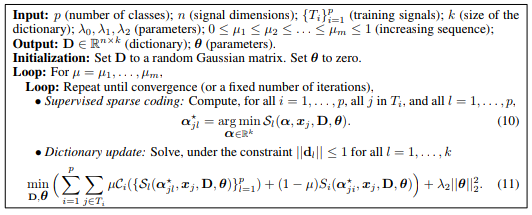
\includegraphics[scale=0.9]{SDL-D.png}
 % SDL-D.png: 532x215 px, 96dpi, 14.07x5.69 cm, bb=0 0 399 161
 \caption{SDL: Supervised dictionary learning Algorithm  \cite{mairal:inria-00322431}}
\end{figure}


